%%
% Please see https://bitbucket.org/rivanvx/beamer/wiki/Home for obtaining beamer.
%%
\documentclass[xcolor=dvipsnames]{beamer} 
\usepackage{graphicx}
\usetheme{Frankfurt}
\setbeamertemplate{items}[circle]
\setbeamertemplate{bibliography item}[text]

% Auto creates the dots for each slide in a section
\usepackage{remreset}
\makeatletter
\@removefromreset{subsection}{section}
\makeatother
\setcounter{subsection}{1}

\usepackage{amsmath}
\usepackage{amssymb}
\usepackage{amsfonts} 
\usepackage{mathtools}
\usepackage{graphicx}
\usepackage{bm}
\usepackage{subcaption}
\usepackage{fancyvrb}
\usepackage{subfigure}
\usepackage{graphicx,xcolor}
\usepackage{pifont,mdframed}
\usepackage{tikz}
\usepackage{bm}
\usetikzlibrary{fit,positioning}


\newcommand \etr[0] {
    \text{etr}
}

\newcommand \Etr[1] {
    \text{etr}\left( { #1 } \right)
}

%
% Macros
%
\newcommand \cashort[1] { {\todo[color=yello]{#1 -- Cedric}} }
\newcommand \calong[1]  { { \todo[inline,color=yellow]{#1 -- Cedric} } }
\newcommand \gbshort[1] { {\todo[color=cyan!40]{#1 -- Guillaume}} }
\newcommand \gblong[1]  { { \todo[inline, color=cyan!40]{#1 -- Guillaume} } }
\newcommand \mgshort[1] { {\todo{#1 -- Mark}} }
\newcommand \mglong[1]  { { \todo[inline]{#1 -- Mark} } }
\newcommand \bfshort[1] { {\todo[color=green!40]{#1 -- Bryan}} }
\newcommand \bflong[1]  { { \todo[inline,color=green!40]{#1 -- Bryan} } }


% Adds a plus const to the end of a math expression
\def \pcst{+\text{const}}

% A fancy version for capital R
\def \Rcal{\mathcal{R}}

% A fancy version for r
\def \rcal{\mathbf{r}}

% Loss function / log likelihood as appropriate
\def \L{\mathcal{L}}

% KL divergence [Math Mode]
\newcommand{\kl}[2] {
	\text{KL}\left[#1||#2\right]
}

\newcommand \vecf[1] {
    \text{vec}\left(#1\right)
}

\newcommand \ent[1] {
    \text{H} \left[ #1 \right]
}

\newcommand \mut[2] {
    \text{I} \left[ #1 ; #2 \right]
}

\newcommand \dvi[2] {
    \text{D}_\text{VI} \left[ #1; #2 \right]
}

% Starts an expected value expresses [Math Mode]
\newcommand{\starte}[1] {%
	\mathbb{E}_{#1}\left[
}

% Ends an expected value expression [Math Mode]
\def \ende{\right]}

% Starts an varianc expresses [Math Mode]
\newcommand{\startv}[1] {%
	\mathbb{V}\text{ar}_{#1}\left[
}

% Ends an variance expression [Math Mode]
\def \endv{\right]}

%\newcommand \ex[2] {
%    \bigl\langle #1 \bigr\rangle_{#2}
%}
\newcommand \ex[2] {
    \mathbb{E}_{ { #2 } }\left[ #1 \right]
}
\newcommand \var[2] {
    \mathbb{V}ar_{ { #2 } }\left[ #1 \right]
}

\newcommand \halve[1] {
	\frac{#1}{2}
}

\newcommand \half {
    \halve{1}
}

\newcommand \tr { \text{tr} } 

\newcommand \T { ^\top } 

\newcommand \fixme[1] {
    {\color{red} FIXME: #1}
}

\newcommand \vv[1] { \boldsymbol #1 }

\newcommand{\mbeq}{\overset{!}{=}}

\newcommand \diag[1] { \text{diag} \left( {#1} \right) }
\newcommand \diagonal[1] { \text{diagonal} \left( {#1} \right) }

\newcommand \Ed {{ \vv{\xi}_d}}
\newcommand \Edj {{\xi_{dj}}}
\newcommand \Edk {{\xi_{dk}}}
\newcommand \AEdj {{\Lambda(\xi_{dj})}}
\newcommand \AEdk {{\Lambda(\xi_{dk})}}
\newcommand \AEd  {{ \bm{\Lambda}(\bm{\xi}_d) }}

\newcommand \Axi { { \Lambda_{\xi} } }
\newcommand \bxi { { \vv{b}_{\xi} } }
\newcommand \cxi { { c_{\xi} } }


\newcommand \wdoc      { { \vv{w}_d } }
\newcommand \wdt[0]  { { w_{dt} } }
\newcommand \wdn[0]  { { \vv{w}_{dn} } }
\newcommand \wdnt[0]  { { w_{dnt} } }
\newcommand \wdd[0]   { { \vv w_{d} } }
\newcommand \zd[0]   { { \vv z_{d} } }
\newcommand \zdn[0]  { { \vv{z}_{dn} } }
\newcommand \zdnk[0] { { z_{dnk} } }
\newcommand \zdk[0]  { { z_{dk} } }
\newcommand \thd[0]  { { \vv \theta_d } }
\newcommand \thdk[0] { { \theta_{dk} } }
\newcommand \thdj[0] { { \theta_{dj} } }
\newcommand \epow[1] { { e^{#1} } }
\newcommand \pkt     { { \phi_{kt}  } }
\newcommand \pk      { { \vv \phi_k } }
\newcommand \lmd     { { \vv \lambda_d } }
\newcommand \lmdk    { { \lambda_{dk} } }
\newcommand \xd      { { \vv x_d } }
\newcommand \atxd     { A ^\top \bm x_d}
\newcommand \axd     { A\bm x_d}
\newcommand \tsq      { { \tau^2 } }
\newcommand \ssq      { { \sigma^2 } }
\newcommand \tmsq     { { \tau^{-2} } }
\newcommand \asq      { { \alpha^2 } }
\newcommand \amsq     { { \alpha^{-2} } }
\newcommand \sgsq     { { \sigma^2 } }
\newcommand \xvec     { { \vv{x} } }
\newcommand \omk      { { \bm \omega _k } }
\newcommand \omkt     { { \omega_{kt} } }
\newcommand \oma     { { \Omega_A } }
\newcommand \gdn      { { \vv{\gamma}_{dn} } }
\newcommand \gdnk     { { \gamma_{dnk} } }
\newcommand \gdk      { { \gamma_{dk} } }
\newcommand \isigt   { { \Sigma^{-1}_{\bm \theta} } }




\newcommand \halfSig { \frac{1}{2\sigma^2} }

\newcommand \nor[2]   { \mathcal{N} \left( {#1}, {#2} \right) }
\newcommand \nord[3]   { \mathcal{N}_{#1} \left( {#2}, {#3} \right) }
\newcommand \mnor[3]  { \mathcal{N} \left(#1, #2, #3\right) }
\newcommand \norp[3]  { \mathcal{N} \left(#1; #2, #3\right) }
\newcommand \mnorp[4] { \mathcal{N} \left(#1; #2, #3, #4\right) }
\newcommand \mul[1]   { \mathcal{M} \left( {#1} \right) }
\newcommand \muln[2]  { \mathcal{M} \left( {#1},{#2} \right) }
\newcommand \dir[1]   { \mathcal{D} \left( {#1} \right) }
\newcommand \pois[1]  { \mathcal{P} \left( {#1} \right) }
\newcommand \gp[2]    { \mathcal{GP} \left( {#1}, #2 \right) }
\newcommand \dir[1]   { \mathcal{D} \left( {#1} \right) }
\newcommand \gam[2]   { \mathcal{G} \left( {#1}, {#2} \right) }
\newcommand \beta[1]  { \mathcal{B}eta \left( {#1}, {#2} \right) }

\newcommand \lne[1]  { { \ln \left( 1 + e^{ #1 } \right) } }
\newcommand \Tr[1]   { \tr \left(  {#1}  \right) }

\newcommand \roud  { \vv{\rho}_{d}  }
\newcommand \rodk { \rho_{dk} }

\newcommand \exA[1]  { \ex{#1}{q(A)} }
\newcommand \exV[1]  { \ex{#1}{q(V)} }
\newcommand \exT[1]  { \ex{#1}{q(\Theta)} }
\newcommand \extd[1] { \ex{#1}{q(\thd)} }
\newcommand \exTV[1] { \ex{#1}{q(\Theta)q(V)} }

\newcommand \Real[0]  { { \mathbb{R} } }
\newcommand \VReal[1] { { \mathbb{R}^{#1} } }
\newcommand \MReal[2] { { \mathbb{R}^{#1 \times #2} } }
\newcommand \Nat[0]  { { \mathbb{N} } }
\newcommand \VNat[1] { { \mathbb{N}^{#1} } }
\newcommand \MNat[2] { { \mathbb{N}^{#1 \times #2} } }

\newcommand \inv[1] { {#1}^{-1} }
\newcommand \invb[1] { \inv{\left( #1 \right)} }

\newcommand \cn { \textsuperscript{\texttt{[{\color{blue}Citation Needed}]}} }

\newcommand \const { { \text{c} } }

\providecommand \floor [1] { \left \lfloor #1 \right \rfloor }
\providecommand \ceil [1] { \left \lceil #1 \right \rceil }


\newcommand \vt[2] { { #1^{(#2)} } }

\newcommand \hashtag[1] { { \ttfamily \##1 } }

\newcommand \mvy  { \vv{m}_{\vv{y}} }
\newcommand \sigvy { { S_Y } }

\newcommand \mmy  { M_Y      }
\newcommand \md   { \vv{m}_d }
\newcommand \phin { \vv{\phi}_n }
\newcommand \isigma { { \inv{\Sigma} } }

\newcommand \sigv     { { \Sigma_V } }
\newcommand \isigv     { { \Sigma^{-1}_V } }

\newcommand \sigy { { \Sigma_Y } }
\newcommand \isigy { { \Sigma_{-1}_Y } }


\newcommand \omy  { { \Omega_Y } }
\newcommand \iomy { { \inv{\Omega_Y} } }

\newcommand \siga     { { \Sigma_A } }
\newcommand \isiga     { { \Sigma^{-1}_A } }
\newcommand \diagv { { \diag{\nu_1,\ldots,\nu_P} } }

\newcommand \ma { \vv{m}_a }
\newcommand \my { \vv{m}_y }

\newcommand \VoU { V \otimes U }

%\newcommand \one { \mathbb{1} }
\newcommand \one  {{  \mathds{1} }}

\newcommand \lse { \text{lse} }
%\newcommand \lse[0] { \mathrm{lse} }

% Conditional independence 
\def\ci{\perp\!\!\!\perp} % from Wikipedia



% ------ For the eval section

% Multinomial PDF [Math Mode]
% params: 1 - the variable
%         2 - the value
%         3 - the state indicator (e.g. k for a distro with K values)
%         4 - any additional subscript
\newcommand{\mpdf}[4] {
	\prod_{#3} {#1}_{{#4} {#3}} ^ {#2}
}

% Dirichlet PDF [Math Mode]
% params: 1 - the variable
%         2 - the hyper-parameter
%         3 - the state indicator (e.g. k for a distro with K values)
%         4 - any additional subscript
\newcommand{\dpdf}[4] {
	\frac{1}{B({#2})} \prod_{#3} {#1}_{{#4} {#3}} ^ {({#2}_{#3} - 1)}
}

% To simplify the sampling equations, this is indicates
% that the given value has had datapoint "m" stripped out
%
\newcommand{\lm}[1] {
	#1^{\setminus m}
}

\newcommand \model[0] {
    \mathcal{M}
}

\newcommand \perplexity[1] {
    \mathcal{P} \left( { #1 } \right)
}

\newcommand \WTrain {
    \mathcal{W}^{(t)}
}

\newcommand \WQuery {
    \mathcal{W}^{(q)}
}

\newcommand \oneover[1] {
    \frac{1}{ {#1} }
}

\newcommand \samp[1] {
    { #1 }^{(s)}
}

\newcommand \etd[0] {
    \vv{\eta}_d
}



\author{Bryan Feeney} 
\institute{Cognitive Match}
\title[Multitask Admixture Prediction]{Multi-Task Learning of Component Strengths in Non-Conjugate Admixture Models}
\institute[University College London]{
  Read this presentation online at: \\
  $\text{ }$\  $\text{ }$\\
  \texttt{http://tinyurl.com/bryansphd2014}\\
  $\text{ }$\\
  $\text{ }$\\

  \texttt{bryan.feeney@ucl.ac.uk}
}
\date[October 2013]{October , 2014}

\begin{document}

%--- the titlepage frame -------------------------%


\begin{frame}[plain]
  \titlepage
\end{frame}




%--- Research - MTL -------------------------%



\begin{frame}{Research}
Three Components
\only<1,2> {
    \begin{enumerate}
        \item Multi-Task Learning
        \item Admixture Modelling ("Topic Models")
        \item Local Variational Bounds
    \end{enumerate}
}

\only<2> {
    \bigskip
    \texttt{http://tinyurl.com/bryansphd2014}
}

\only<3> {

    \begin{enumerate}
        \item { \bf Multi-Task Learning }
        \item {\color{gray} Admixture Modelling ("Topic Models")}
        \item {\color{gray} Local Variational Bounds}
    \end{enumerate}


}
\end{frame}


%--- ---- MTL -------------------------%


\section{Multi Task Learning}
\begin{frame}{Multi-Task Learning}
Problem: Making many predictions from the same idea
\begin{enumerate}
    \item Predict exam scores in $L$ subjects for several children\cite{Bonilla2008}
    \item Predict customers affinity to $L$ observed aspects of a product\cite{Allenby1999}
    \item Propose image captions by predicting p(word|image) from image features for $L$ words (in this case $L > 10,000$)\cite{Archambeau2011}
\end{enumerate}

\medskip 
\pause

Key ideas codified in \cite{Caruana1997}
\begin{enumerate}
    \item Learn correlations between tasks.
    \item Learn structure of features by how we use them - via regularization
    \item Learn a low-rank projection of the tasks themselves
\end{enumerate}
\end{frame}


%--- Regularization -------------------------%



\begin{frame}{Regularization}

\only<1->{
Learn $L$ vectors $\vv{w}_l$. How to \emph{transfer} knowledge from inferring $\vv{w}_1, \ldots, \vv{w}_{l-1}$ to the task of inferring $\vv{w}_l$
}

\medskip 

\only<2>{

    \begin{equation*}
    y_{nl}|\vv{w}_l & \sim \nor{\vv{w}_l\T\vv{x}_n}{\sigma^2 I} & \qquad
        \vv{w}_l & \sim \nor{\vv{0}}{\alpha^2 I} 
    \end{equation*}

}

\only<3>{
    Bayesian approach - learn the prior\cite{Allenby1999}
    
    \begin{align*}
        y_{nl}|\vv{w}_l & \sim \nor{\vv{w}_l\T\vv{x}_n}{\sigma^2 I} & \qquad
        \vv{w}_l & \sim \nor{\vv{m}}{\Sigma} \\
        \vv{m}|\Sigma & \sim \nor{\vv{m}_0}{\oneover{\lambda}\Sigma} & \qquad
        \Sigma & \sim \mathcal{W}^{-1}\left(\Sigma_0, \nu\right)
    \end{align*}
}

\only<4>{
    Exploit sparsity using ARD priors
    
    \begin{align*}
        y_{nl}|\vv{w}_l & \sim \nor{\vv{w}_l\T\vv{x}_n}{\sigma^2 I} & \qquad
        \vv{w}_l & \sim \nor{\vv{0}}{\diag{\vv{\alpha}}} \\
        \alpha_f & \sim \mathcal{G}\left( a, b \right)
    \end{align*}
}

\only<5>{
    Exploit sparsity using Clustered ARD priors\cite{BakkerHeskes2003}
    
    \begin{align*}
        y_{nl}|\vv{w}_l & \sim \nor{\vv{w}_l\T\vv{x}_n}{\sigma^2 I} & \qquad
        \vv{w}_l|z_{l} & \sim \nor{\vv{0}}{\diag{\vv{\alpha}_{z_l}}} \\
        z_l & \sim \muln{\vv{\theta}}{1} &
        \alpha_{fk} & \sim \mathcal{G}\left( a, b \right) \\
        \vv{\theta} & \sim \dir{\beta}
    \end{align*}
}

\only<6>{
    Low-Rank Projections of the Feature Space  
    \begin{align*}
        y_{nl}|\vv{w}_l & \sim \nor{\vv{w}_l\T\vv{x}_n}{\sigma^2 I} & \qquad
        \vv{w}_l|\vv{z} & \sim \nor{U \vv{z}_l}{\alpha^2 I} \\
        & & \qquad \vv{z}_l & \sim \nor{\vv{0}}{I} \\
        \implies \vv{w}_l & \sim \nor{\vv{0}}{\alpha^2 I + U U\T}  
    \end{align*}
}

\only<7>{
    This is all just hierarchical Bayeisan modelling\\
    \medskip
    However analogous methods exist in error-optimisation approaches to machine learning which learn regularization functions instead of priors.
    \begin{itemize}
        \item Heterogeneous sparsity in \cite{Argyriou2005}
        \item Low-Rank projections in \cite{argyriou2007spectral}
    \end{itemize}

}

\end{frame}


%--- Regularization and Correlation -------------------------%

\begin{frame}{Regularization and Correlation}
Once can also take into account task correlation by setting $W = \left\{ \vv{w}_l \right\}_{l=1}^L$ (note $W \in \MReal{L}{F}$), and defining

\begin{align*}
    \vv{y}_n|W & \sim \nor{W\vv{x}_n}{\Omega} & \vv{w}_l \sim \prod_l \nor{0}{\Sigma}
\end{align*}

where $\Omega \in \MReal{L}{L}$ is the \emph{task} correlation, $\Sigma \in \MReal{F}{F}$ is the \emph{feature} correlation, and these are learnt in the usual manner.


\end{frame}

%--- Matrix Variate Prior -------------------------%

\begin{frame}{Matrix-Variate Priors}
Matrix-Variate Normal Distribution \cite{Gupta1999} :
\begin{align*}
W \sim \mnor{M}{\Omega}{\Sigma} & \implies \vecf{W} \sim \nor{\vecf{M}}{\Sigma \otimes \Omega}
\end{align*}

{ \fontsize{9}{11}\selectfont
\begin{align*}
\ln p(W) = -\halve{FL} \ln 2\pi - \halve{F}\ln |\Omega| - \halve{L} \ln | \Sigma | - \half \text{etr} \left( \inv{\Sigma} (W - M) \inv{\Omega} (W - M)\T \right)
\end{align*}
}
where $\text{etr}(X) = \exp \left( \Tr{X} \right)$\\

\bigskip
\pause
Matrix Variate Priors for Multi-Task Learning\cite{Bonilla2008}\cite{Archambeau2011}
, infer $Y \in \MReal{D}{L}$ from $X \in \MReal{D}{F}$

\begin{align*}
Y | W & \sim \mnor{XW}{I_D}{\Sigma} & \quad W \sim \mnor{0}{\Omega}{\Sigma} \\
Y &\sim \mnor{0}{I_D + X \Omega X\T}{\Sigma}
\end{align*}
Defining a multi-task Gaussian Process regression model\cite{Bonilla2008}.

\end{frame}

%--- Research -------------------------%

\section{Admixture Modelling}

\begin{frame}{Research}
Three Components


    \begin{enumerate}
        \item { \color{gray} Multi-Task Learning }
        \item { \bf Admixture Modelling ("Topic Models")}
        \item {\color{gray} Local Variational Bounds}
    \end{enumerate}


\end{frame}

%--- Admixture Modelling -------------------------%

\begin{frame}{Mixture Models versus Admixture Models}

\only<1,2,6,8,9>{
Classical Mixture Model of Text - One topic per document
\begin{align*}
\vv{\theta} & \sim \dir{\alpha} & z_d & \sim \muln{\vv{\theta}}{1} & w_{dn} \sim \muln{\vv{\phi}_{z_d}}{1}
\end{align*}
Where each of the component vocabularies is drawn $\vv{\phi}_k \sim \dir{\vv{\beta}}$.
}

\medskip

\only<2>{
However in practice this is not what people actually do...
}

\only<3>{ 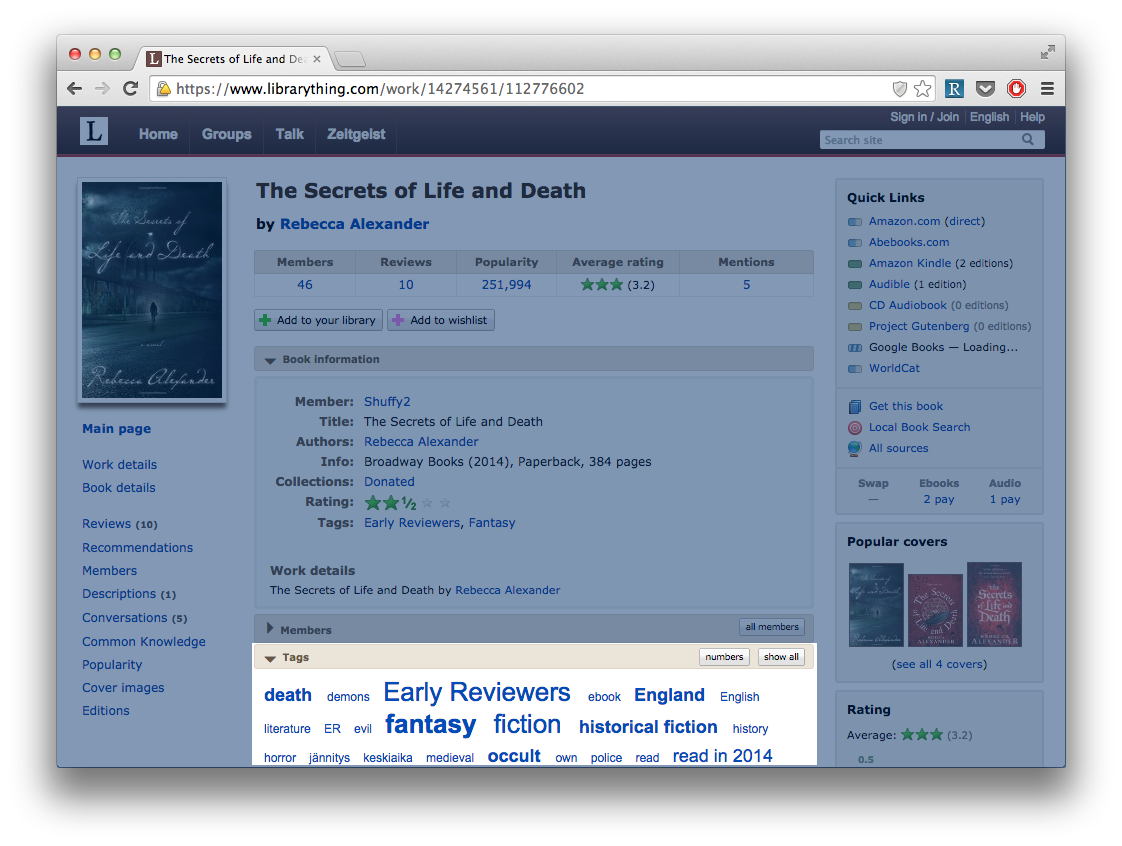
\includegraphics[width=1\textwidth]{images/BookTags.png}}
\only<4>{ 
\includegraphics[width=1\textwidth]{images/NetflixTags.png}}
\only<5>{ 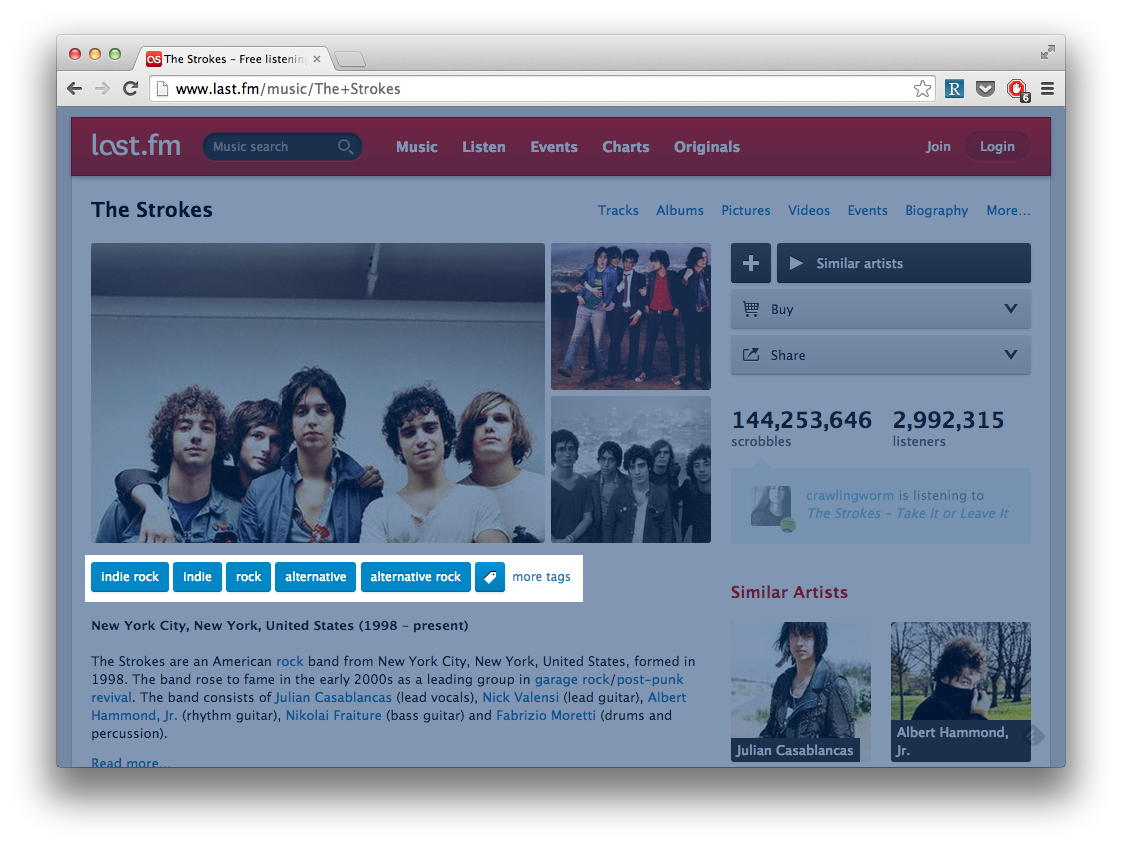
\includegraphics[width=1\textwidth]{images/lastfmTags.png}}

\only<6> {
Mixture models struggle to generalise.
\begin{itemize}
    \item Fewer clusters mean coarser estimates of cluster centroids
    \item But more clusters mean fewer datapoints per cluster, and thus sparser estimates of cluster centroids (for text), due to the assumption of one cluster per document
\end{itemize}
}

\only<7> {
    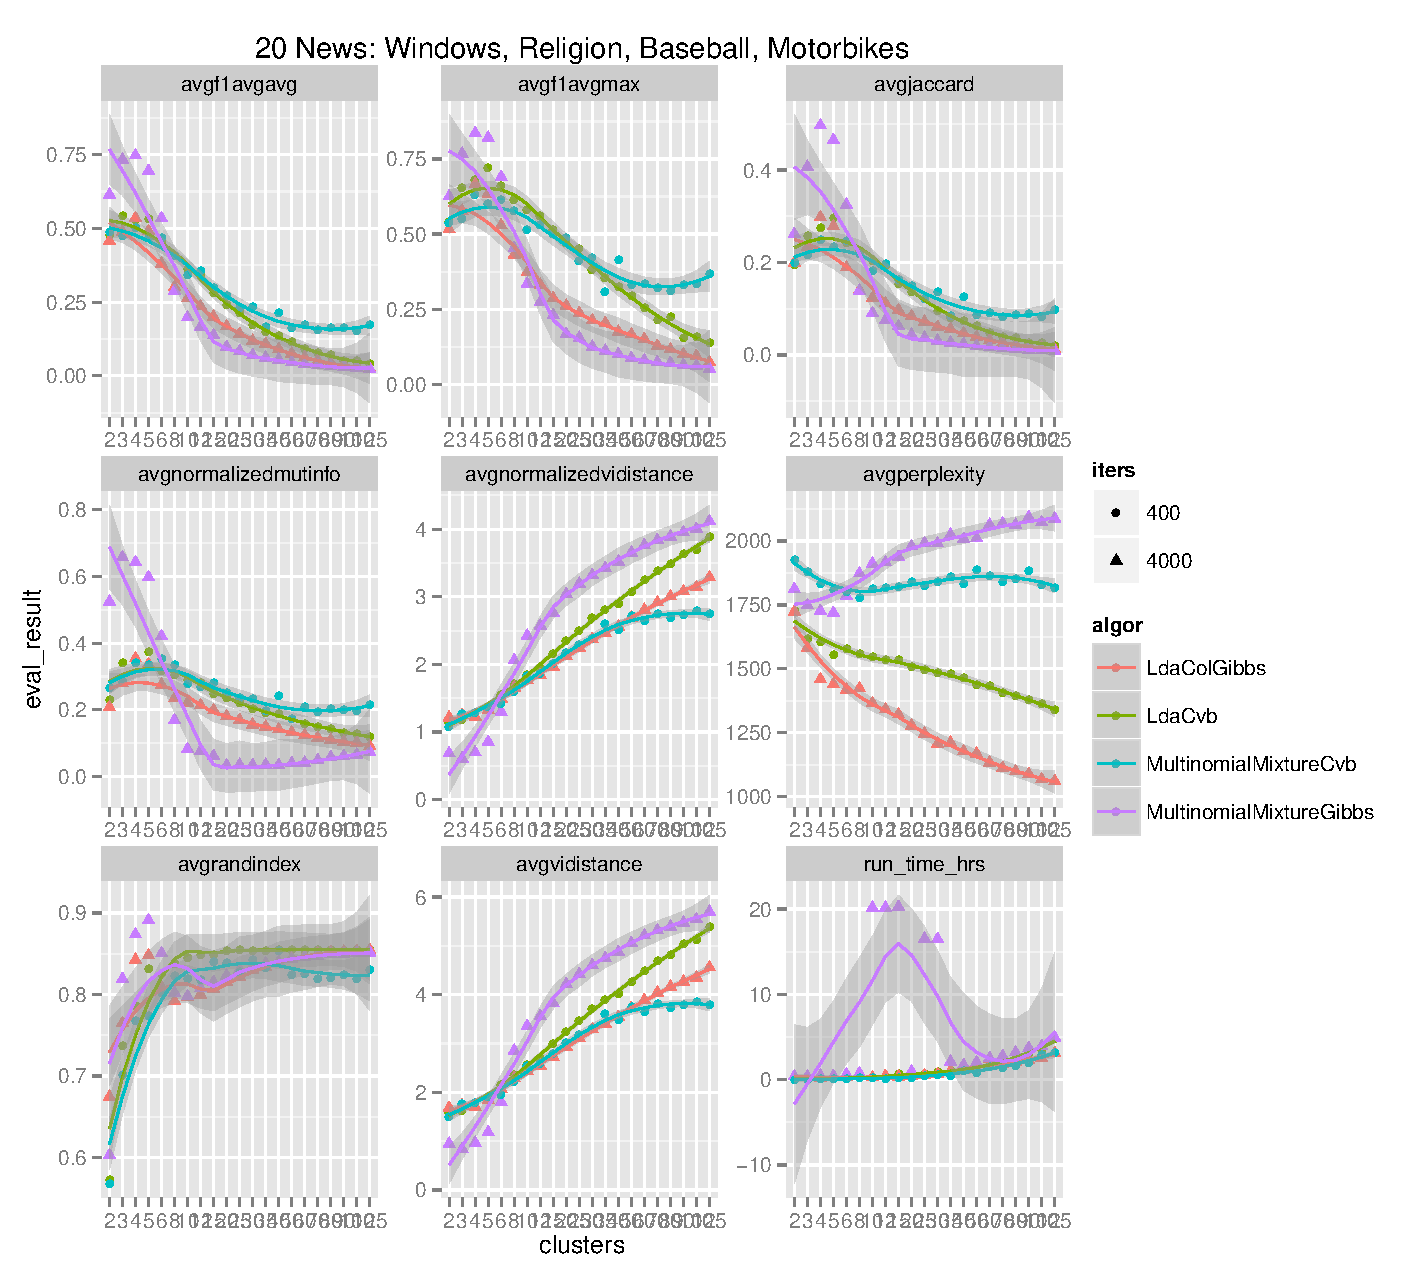
\includegraphics[trim=12.3cm 7.3cm 0.5cm 7.7cm, clip=true, totalwidth=0.8\textwidth]{Images/20news-2013-03-25.pdf}
}

\only<8> {
Admixture models assign a \emph{mixture} of topics to each document, 

In the case of text the ``topic-model" implementation\cite{BleiNgJordan2003} assigns a single topic to each word $w_{dn}$.

\begin{align*}
\vv{\theta}_d & \sim \dir{\alpha} & z_{dn} & \sim \muln{\vv{\theta}_d}{1} & w_{dn} \sim \mul{\vv{\phi}_{z_{dn}},1}
\end{align*}

}

\only<9> {
Sample colored text
}


\end{frame}

%--- Topic Model Relationships --------------------%

\begin{frame}{Topic Models: Multinomial Admixtures}
Links to other models
\begin{itemize}
    \item<1->Multinomial PCA
    \only<1>{
        \begin{itemize}
            \item Drop the prior on the component distributions, treat $\vv{\phi}_k$ as a parameter
            \item Collect into a single $T \times K$ matrix $\Phi = \{ \vv{\phi}_k \}_{k=1}^{K}$
            \item Can now represent a document as a projection of a latent low-dimensional document
            \begin{align}
                \wdoc & \sim \muln{\Phi \thd}{n_d} & \thd &\sim \dir{\alpha}
            \end{align}
            \item From which the correspondence to PCA should be clear
            \begin{align}
                \xd & \sim \nor{A \vv{z}_d}{\sigma^2 I} & \vv{z}_d \sim \nor{0}{I}
            \end{align}


        \end{itemize}
    
    }
    
    \item<2->(Non-Negative) Matrix Factorization
    \only<2> {
        \begin{itemize}
            \item Collect the topic probabilities into the $D \times K$ matrix $\Theta = \{ \thd\T \}_{d=1}^D$
            \item Account for document length by letting $\hat{\Theta} = \diag{n_1, n_2, \ldots, n_D} \Theta$
            \begin{align}
                W \approx  \hat{\Theta}\Phi\T
            \end{align}
            \item Can do this directly by using $K\times T$ independent Poisson distributions instead of $K$ Mulitnomials $\vv{\phi}_k$, with corresponding Gamma priors\cite{Gopalan2013}

        \end{itemize}
    }
    \only<3> { \smallskip }
\end{itemize}

\end{frame}



%--- Topic Model Research -------------------------%

\begin{frame}{Topic Models: Multinomial Admixtures}
Five broad areas of research
\begin{itemize}
    \item<1-> Richer Observation Models
        \only<1> { \begin{itemize}
        \item Language Models\cite{Wallach2006}\cite{Wang2007}\cite{Lindsey2012} 
        \item Alternative distrbutions such as logistic-normal\cite{Blei2006a}\cite{Eisenstein2010} or von Mises - Fisher\cite{Reisinger2010}
    \end{itemize} }
    
    \item<2-> Alternatives to the Dirchlet prior
    \only<2> { 
        \begin{itemize}
            \item The ``Logistic Normal" prior for the Correlated Topic Model\cite{Blei2006}
        \end{itemize}

        \begin{align}
        \vv{\eta}_d & \sim \nor{\mu}{\Sigma} \\
        \theta_{dk} & = \frac{\exp(\eta_{dk})}{\sum_j \exp(\eta_{dj})} \\
        \implies \ln \theta_{dk} & = \eta_{dk} - \log(\sum_j \exp(\eta_{dj}) \\
         & = \eta_{dk} - \lse(\vv{\eta}_d)
    \end{align} 
    }

    \item<3-> Bayesian Non-Parametrics to estimate Topic Counts
    \only<3> { \begin{itemize}
         \item Hierarchical Dirichlet Processes\cite{Teh2006b}
         \item Discrete Infinite Logistic Normal Distribution\cite{Paisley2012}
    \end{itemize} }

    \item<4-> Scalable Implementations: 
    \only<4> { \begin{itemize}
        \item Gibbs Sampling\cite{Pritchard2000} and Collapsed Gibbs Sampling\cite{Griffiths2004} 
        \item Variational\cite{BleiNgJordan2003} inference and Collapsed Variational\cite{Teh2007}\cite{Hensman2012} inference
        \item MAP and other approximations\cite{Asuncion2012}
        \item Distributed "Big Data" approaches\cite{Smola2010}\cite{Newman2009}\cite{Chen2013}
        \item Optimised online approaches\cite{Hoffman2010}\cite{Hoffman2012}\cite{Mimno2012a}
    \end{itemize} }
    
    \item<5-> Use of Covariates $\vv{x}_d$
    \only<5> { \begin{itemize}
        \item Ad-hoc Models: topics over time\cite{Wang2006}, author-topics\cite{MacCallum2007}, regional topics\cite{Eisenstein2010}
        \item ``Downstream" Models\cite{Blei2003}\cite{Salomatin2009}\cite{Virtanen2012a} \\$\qquad p(\wdoc,\xd) = \int_{\thd} p(\wdoc|\thd) p(\xd|\thd) p(\thd)$.
        \item ``Upstream" Models:\cite{Mimno2008} $p(\wdoc | \xd) = \int_{\thd} p(\wdoc|\thd) p(\thd|\xd)$.
    \end{itemize} 
    }
    
    \only<6>{\medskip}
\end{itemize}


\end{frame}

\section{Local Variational Bounds}

\begin{frame}{Research}
Three Components


    \begin{enumerate}
        \item { \color{gray} Multi-Task Learning }
        \item { \color{gray} Admixture Modelling ("Topic Models")}
        \item { \bf Local Variational Bounds}
    \end{enumerate}


\end{frame}


%--- Local Variational Intro -------------------------%


\begin{frame}{Local Variational Bounds}

The softmax transformation
\begin{align}
    \ln \sigma_k\left(\thd\right) = \eta_{dk} - \lse(\vv{\eta}_d)
\end{align}
Problems
\begin{itemize}
    \item Prior (a Gaussian) is not conjugate to the likelihood (a multinomial mixture)
    \item No analytic form for the posterior.
\end{itemize}
Approach is to approximate the likelihood using bounds
\begin{itemize}
    \item Classic approach is a global bound over the entire likelihood (e.g. the Laplace approximation)
    \item A better fit, and more flexibility, can be obtained by using \emph{local} bounds over the likelihood of each document.
\end{itemize}

\end{frame}

%--- Bounds List -------------------------%


\begin{frame}{Local Variational Bounds}

\begin{itemize}
    \item Global Bounds: Laplace, Delta Method\cite{Wang2013a}
    \item Quadratic Bounds: Bohning\cite{Bohning1988a}, Bouchard\cite{Bouchard2007}
    \item Other more recent bounds
    \begin{itemize}
        \item Piecewise Quadratic Bounds\cite{Marlin2011}
        \item Tilted Bound\cite{MinkaKnowles}
        \item Stick-breaking bound\cite{Khan2012stick}
    \end{itemize}
\end{itemize}


\end{frame}


%--- Research -------------------------%

\section{Research}
\begin{frame}{Research}

Current Project
\begin{itemize}
    \item Predicting component strengths for upstream topic-models
    \item Employing matrix-variate prior over weights to jointly
    \begin{itemize}
        \item Capture correlations between topics
        \item Capture a low-rank projection of the feature-covariance
        \item Topic Model itself captures a low-rank representation of word-counts        
    \end{itemize}
\end{itemize}

Use-Cases: Microtexts
\begin{itemize}
    \item Tweets: Predict text given user features (username, time tweet was posted). Notably predict absent words such as \strong{hashtags}.
    \item Image captions: Predict caption given image features.
\end{itemize}

\end{frame}


%--- Model -------------------------%

\begin{frame}{Model}

The Model
\begin{align}
Z & \sim \mnor{0}{I}{I} & A|Z & \sim \mnor{AZ}{I}{\Sigma} \\
\vv{\eta}_d & \sim \nor{A\xd}{\Sigma} & \thd & = \vv{\sigma}(\vv{\eta}_d) \\
z_{dn} & \sim \muln{\thd}{1} & w_{dn} & \sim \muln{\vv{\phi}_{z_{dn}}}{1} 
\end{align}

Inference
\begin{itemize}
    \item Use quadratic bounds to approximate the per-document likelihoods
    \item Use the variational bound to approximate the posterior using a meanfield approximation of the posterior $q(Z, \Phi, \Theta) \approx q(Z)q(\Theta)q(\Phi)$
\end{itemize}


\end{frame}

%--- Datasets -------------------------%

\begin{frame}{Model}

Two Datasets
NIPS Papers from 1987 to 1999
\begin{itemize}
    \item 682 Documents. Vocabulary of 12503 words
    \item Median document length of 1,532 words, total of 1,075,323 words across the corpus
    \item Features are: authors; citations; {\color{gray} the year}
\end{itemize}

Tweets from April to September 2013 (inclusive)
\begin{itemize}
    \item 735,868 tweets from 572 users. Vocabulary of 82,698 words
    \item Median tweet length is 10 words (genuinely!), total of 7,272,228 word observations across the corpus 
    \item Features are: authors; time at various granularities (hour, day, week, month)
\end{itemize}

Images are ongoing

\end{frame}

%--- Datasets -------------------------%

\begin{frame}{Model}

Two Datasets
NIPS Papers from 1987 to 1999
\begin{itemize}
    \item 682 Documents. Vocabulary of 12503 words
    \item Median document length of 1,532 words, total of 1,075,323 words across the corpus
    \item Features are: authors; citations; {\color{gray} the year}
\end{itemize}

Tweets from April to September 2013 (inclusive)
\begin{itemize}
    \item 735,868 tweets from 572 users. Vocabulary of 82,698 words
    \item Median tweet length is 10 words (genuinely!), total of 7,272,228 word observations across the corpus 
    \item Features are: authors; time at various granularities (hour, day, week, month)
\end{itemize}

Images
\begin{itemize}
    \item Ongoing
\end{itemize}

\end{frame}


%--- Results -------------------------%

\begin{frame}{Model}

Two Datasets
NIPS Papers from 1987 to 1999
\begin{itemize}
    \item 682 Documents. Vocabulary of 12503 words
    \item Median document length of 1,532 words, total of 1,075,323 words across the corpus
    \item Features are: authors; citations; {\color{gray} the year}
\end{itemize}

Tweets from April to September 2013 (inclusive)
\begin{itemize}
    \item 735,868 tweets from 572 users. Vocabulary of 82,698 words
    \item Median tweet length is 10 words (genuinely!), total of 7,272,228 word observations across the corpus 
    \item Features are: authors; time at various granularities (hour, day, week, month)
\end{itemize}

Images
\begin{itemize}
    \item Ongoing
\end{itemize}

\end{frame}


%--- the Bibliography frame -------------------------%

\section{Reference}
\begin{frame}[allowframebreaks]{Reference}


\bibliographystyle{plain}
\bibliography{/Users/bryanfeeney/Documents/library.bib}


\end{frame}



\end{document}